\section{RDF, OWL, and serialization formats}
\label{sec:rdf-owl-formats}

%% RDF
The \acf{RDF} is a \ac{W3C} graph-based standard model to represent information about resources on the Web (including documents, people, physical objects, and abstract concepts). Using \ac{RDF}, machines can process information on the Web using common parsers and processing tools, and information can be exchanged between different applications without losing meaning \cite{world2014rdfprimer}. In particular, in recent years \ac{RDF} has become the \textit{de-facto} standard for publishing Linked Data on the Web. The core structure of the \ac{RDF} syntax is a set of statements, called \textit{triples}, because they consist of three elements: a \textit{subject}, a \textit{predicate}, and an \textit{object}, following the structure \verb#<subject> <predicate> <object>#, which can be visually represented in Figure \ref{fig:rdf-graph-structure} \cite{world2014rdfconcepts}.

\begin{figure}[!ht]
    \centering
    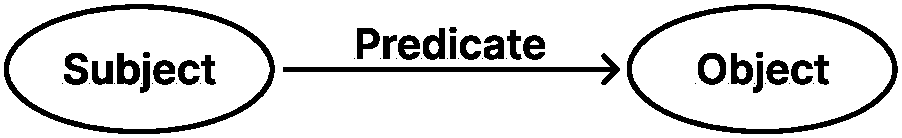
\includegraphics[width=0.55\columnwidth]{images/rdf-graph-structure.pdf}
    \caption{The structure of a triple, with two nodes and a predicate connecting them.}
    \label{fig:rdf-graph-structure}
\end{figure}

The subject and the object represent the two resources being related. The relationship that goes from the subject to the object is called \textit{property}, and its nature is represented by the predicate. A set of statements generate a direct graph, called RDF graph, where subjects and objects are the nodes of the graph, and the predicates form the arcs. For example, the set of triples below produces the graph shown in Figure \ref{fig:rdf-graph-examle} \cite{world2014rdfprimer}.

\begin{verbatim}
<Bob> <is a> <person>.
<Bob> <is a friend of> <Alice>.
<Bob> <is born on> <the 4th of July 1990>.
<Bob> <is interested in> <the Mona Lisa>.
<the Mona Lisa> <was created by> <Leonardo da Vinci>.
<the video 'La Joconde à Washington'> <is about> <the Mona Lisa>
\end{verbatim}

\begin{figure}[!ht]
    \centering
    \includegraphics[width=0.95\columnwidth]{images/rdf-graph-example.pdf}
    \caption{The example of the \ac{RDF} graph presented by \ac{W3C}.}
    \label{fig:rdf-graph-examle}
\end{figure}

In an \ac{RDF} graph, resources may be represented using an \ac{IRI}, a \textit{literal value} or a \textit{blank node}. An \ac{IRI} is a generalization of \ac{URI}, where non-\acs{ASCII} characters are allowed in the \ac{IRI} character string. \acp{IRI} identify resources, and can appear in all three positions of a triple. In the example above, the \ac{IRI} for Leonardo Da Vinci in DBpedia\footnote{\url{https://www.dbpedia.org/}} is \url{http://dbpedia.org/resource/Leonardo_da_Vinci}.

Literals are basic values such as strings, dates, and numbers. In the \ac{RDF} graph literals can only be used as objects, and consists of two or three elements, which are: (1) the value itself; (2) an \ac{IRI} that identifies the \textit{datatype} (string, number, date, etc.); (3) if and only if the datatype is a \texttt{rdf:langString},\footnote{\url{http://www.w3.org/1999/02/22-rdf-syntax-ns\#langString}} a \textit{language tag} (such as \texttt{en}, \texttt{it}, \texttt{fr}, etc.) \cite{world2014rdfconcepts}.

Finally, blank nodes can appear in the subject and object position of a triple and are used to represent resources without using a \ac{IRI} \cite{world2014rdfprimer}.

%% OWL
\paragraph*{}
In Section \ref{sec:web-of-data} ontologies and vocabularies are presented as a core element for creating the Semantic Web. The \ac{RDF} data model does not provide semantic information about the resources. For this reason, \ac{RDF} provides the \ac{RDFS} language, that allows to define semantic characteristics of data. \acl{RDFS} uses the notion of \textit{class} to classify resources, while uses the \textit{type} property to define a relation between an instance and its class. \acl{RDFS} also allows defining type restrictions on subject and objects of particular triples through \textit{domain} and \textit{range} restrictions. Finally, with \acl{RDFS} it is also possible to define hierarchies of classes and properties, using \textit{subClassOf} and \textit{subPropertyOf} predicates \cite{world2014rdfprimer}. All of these modeling constructs provided by \acl{RDFS} are summarized in Table \ref{tab:rdfs-constructs}.

\begin{table}[!ht]
    \centering
    \doublespacing
    \begin{tabular}{|l|l|l|}
        \hline
        \multicolumn{1}{|c|}{\textbf{Construct}} & \multicolumn{1}{c|}{\textbf{Syntactic form}} & \multicolumn{1}{c|}{\textbf{Description}}            \\ \hline
        \textbf{Class}                           & C rdf:type rdfs:Class                        & C is an RDF class                       \\ \hline
        \textbf{Property}                        & P rdf:type rdf:Property                      & P is an RDF property                    \\ \hline
        \textbf{type}                            & I rdf:type C                                 & I is an instance of C         \\ \hline
        \textbf{subClassOf}                      & C1 rdfs:subClassOf C2                        & C1 is a subclass of C2           \\ \hline
        \textbf{subPropertyOf}                   & P1 rdfs:subPropertyOf P2                     & P1 is a sub-property of P2 \\ \hline
        \textbf{domain}                          & P rdfs:domain C                              & domain of P is C             \\ \hline
        \textbf{range}                           & P rdfs:range C                               & range of P is C              \\ \hline
    \end{tabular}
    \caption{The main modeling constructs provided by RDF Schema.}
    \label{tab:rdfs-constructs}
\end{table}

However, in 2004 the \acl{W3C} presented \ac{OWL}, a more complete language for publishing and sharing ontologies on the Web \cite{bechhofer2004owl}, and replaced in 2009 and then in 2012 by \ac{OWL} 2. \ac{OWL} 2 is a Semantic Web language to represent rich and complex knowledge about things, groups of things, and relations between things. In addition, since \ac{OWL} is a computational logic-based language, the knowledge expressed in \ac{OWL} can be reasoned with by computer programs either to verify the consistency of that knowledge or to make implicit knowledge explicit. A \ac{OWL} document, called \textit{ontology}, can be published in the World Wide Web and may refer to or be referred from other \ac{OWL} ontologies \cite{hitzler2009owl}. In \ac{OWL} 2 knowledge is represented by statements, called \textit{axioms}. Axioms normally refer to objects of the world and describe them by putting them into categories or saying something about their relation. In \ac{OWL} 2 objects, categories and relations are called \textit{entities}, and in particular objects are denoted as \textit{individuals}, categories as \textit{classes} and relations as \textit{properties}. Moreover, properties are further subdivided into (1) \textit{object properties} that relate objects to objects; (2) \textit{datatype properties} that assign data values to objects; (3) \textit{annotation properties} that encode information about the ontology itself. Finally, names of entities can be combined into \textit{expressions} using \textit{constructors} to form complex descriptions from basic ones \cite{hitzler2009owl}.

\paragraph*{}
In order to publish \ac{RDF} data on the Web, the \ac{RDF} graphs need to be serialized. Today there are several serialization formats, but the most famous one are: N-Triples, Turtle, RDF/XML, RDFa, and JSON-LD. These formats are briefly described below, reporting as example of small excerpt of DBpedia\footnote{\url{https://www.dbpedia.org/}} is reported.

\paragraph*{N-Triples\footnote{\url{https://www.w3.org/TR/n-triples/}}} It's one of the simplest formats, formed by sequences of \ac{RDF} triples. Each statement is formed by the subject, predicate, object, and a ".", that are separated by white space.

\begin{verbatim}
<http://dbpedia.org/page/Jotaro_Kujo>
  <http://dbpedia.org/ontology/relative>
    <http://dbpedia.org/page/Joseph_Joestar> .
\end{verbatim}

\paragraph*{Turtle\footnote{\url{https://www.w3.org/TR/turtle/}}} It's a common data format for serializing \ac{RDF} graphs that introduces some features to N-Triples language. In particular, it introduces the use of \texttt{@base} \ac{IRI} and relative \acp{IRI}, \texttt{@prefix} and prefixed names, predicate lists separated by ";", object lists separated by ",", and the representation of \texttt{rdfs:type} with the token \texttt{a}.

\begin{verbatim}
@prefix dbr: <http://dbpedia.org/page/> .
@prefix dbo: <http://dbpedia.org/ontology/> .

dbr:Jotaro_Kujo dbo:relative dbr:Joseph_Joestar .
\end{verbatim}

\paragraph*{RDF/XML\footnote{\url{https://www.w3.org/TR/rdf-syntax-grammar/}}} Expresses \ac{RDF} graphs as an \acs{XML} document. The nodes and predicates are represented in \acs{XML} terms: element names, attribute names, element contents and attribute values.

\begin{verbatim}
<rdf:RDF xmlns:dbr="http://dbpedia.org/page/"
  xmlns:dbo="http://dbpedia.org/ontology/"
  xmlns:rdf="http://www.w3.org/1999/02/22-rdf-syntax-ns#"
  xml:base="http://www.ldf.fi/service/rdf-serializer/">
  <rdf:Description
    rdf:about="http://dbpedia.org/page/Jotaro_Kujo">
    <dbo:relative
      rdf:resource="http://dbpedia.org/page/Joseph_Joestar"/>
  </rdf:Description>
</rdf:RDF>    
\end{verbatim}

\paragraph*{\ac{RDFa}\footnote{\url{https://www.w3.org/TR/rdfa-primer/}}} Provides a set of markup attributes to \acs{HTML} pages to augment the visual information on the Web with machine-readable hints.

\begin{verbatim}
<body
  prefix="dbr: http://dbpedia.org/page/
    dbo: http://dbpedia.org/ontology/">
  <div about="dbr:Jotaro_Kujo">
    <div
      rel="dbo:relative"
      resource="dbr:Joseph_Joestar">
    </div>
  </div>
</body>  
\end{verbatim}

\paragraph*{JSON-LD\footnote{\url{https://www.w3.org/TR/json-ld/}}} Serializes \ac{RDF} graphs into \ac{JSON}. The syntax is designed to easily integrate into deployed systems that already use \ac{JSON}. It's intended to be a way to use Lined Data in Web-based programming environments, to build interoperable Web services, and to store Linked Data in \ac{JSON}-based storage engines.

\begin{verbatim}
[
  {
    "@id": "http://dbpedia.org/page/Joseph_Joestar"
  },
  {
    "@id": "http://dbpedia.org/page/Jotaro_Kujo",
    "http://dbpedia.org/ontology/relative": [
      {
        "@id": "http://dbpedia.org/page/Joseph_Joestar"
      }
    ]
  }
]
\end{verbatim}